\documentclass[10pt,twocolumn,letterpaper]{article}

\usepackage{cvpr}
\usepackage{times}
\usepackage{epsfig}
\usepackage{graphicx}
\usepackage{multirow} % creates cells that span multiple rows in a table
\usepackage{amsmath}
\usepackage{amssymb}
\usepackage{bm} % bold fonts for math symbols
\usepackage{booktabs}
\usepackage[export]{adjustbox} % adds a frame around figures
\usepackage{IEEEtrantools} % IEEEeqnarray math equation environment
\usepackage{multirow} % merge multiple rows
\usepackage{tabularx} % for 'tabularx' environment
\usepackage{caption} % controls spacing between caption and table

% Include other packages here, before hyperref.

% If you comment hyperref and then uncomment it, you should delete
% egpaper.aux before re-running latex.  (Or just hit 'q' on the first latex
% run, let it finish, and you should be clear).
\usepackage[pagebackref=true,breaklinks=true,letterpaper=true,colorlinks,bookmarks=false]{hyperref}

\cvprfinalcopy % *** Uncomment this line for the final submission

\def\cvprPaperID{7245} % *** Enter the CVPR Paper ID here
\def\httilde{\mbox{\tt\raisebox{-.5ex}{\symbol{126}}}}

\newcommand{\bx}{\bm{x}}
\newcommand{\tx}{\tilde{\bm{x}}}
\newcommand{\bX}{\bm{X}}
\newcommand{\by}{\bm{y}}
\newcommand{\bY}{\bm{Y}}
\newcommand{\bq}{\bm{q}}
\newcommand{\bQ}{\bm{Q}}
\newcommand{\bk}{\bm{k}}
\newcommand{\bK}{\bm{K}}
\newcommand{\bv}{\bm{v}}
\newcommand{\bV}{\bm{V}}
\newcommand{\bh}{\bm{h}}
\newcommand{\bH}{\bm{H}}
\newcommand{\bg}{\bm{g}}
\newcommand{\bG}{\bm{G}}
\newcommand{\bb}{\bm{b}}
\newcommand{\bB}{\bm{B}}
\newcommand{\bw}{\bm{w}}
\newcommand{\bW}{\bm{W}}
\newcommand{\bz}{\bm{z}}
\newcommand{\bZ}{\bm{Z}}
\newcommand{\tz}{\tilde{\bm{z}}}
\newcommand{\bd}{\bm{d}}

% Pages are numbered in submission mode, and unnumbered in camera-ready
\ifcvprfinal\pagestyle{empty}\fi
\pagenumbering{gobble}

\begin{document}

%%%%%%%%% TITLE - suggestions and candidates
\title{Transform and Tell: Entity-Aware News Image Captioning\\Supplementary Material}
% \title{Transforming Entities for News Image Captions\\Supplementary Material}

\author{Alasdair Tran, Alexander Mathews, Lexing Xie\\
Australian National University\\
{\tt\small \{alasdair.tran,alex.matthews,lexing.xie\}@anu.edu.au}
% For a paper whose authors are all at the same institution,
% omit the following lines up until the closing ``}''.
% Additional authors and addresses can be added with ``\and'',
% just like the second author.
% To save space, use either the email address or home page, not both
}

\maketitle
%\thispagestyle{empty}

\section{Live Demo}

A live demo of our model is available at
\href{https://transform-and-tell.ml}{https://transform-and-tell.ml}. In the
demo, the user is able to provide the URL to a New York Times article. The
server will then scrape the web page, extract the article and image, and
feed them into our model to generate a caption.

\section{Entity Distribution}

Figure \ref{fig:entities} shows how different name entity types are distributed
in the training captions of the NYTimes800k dataset. The four most popular
types are people's names (PERSON), geopolitical entities (GPE), organizations
(ORG), and dates (DATE). Out of these, people's names comprise a third of all
named entities. This motivates us to add a specialized face attention module to
the model.

%%%%%%%%% BODY TEXT
\section{Model Complexity}

Table \ref{tab:models} shows the number of training parameters in each of our
model variants. We ensure that the total number of trainable parameters for
each model is within 7\% of one another (148 million to 159 million), with the
exception of the model with face attention (171 million) and with object
attention (200 million) since the latter two have extra multi-head attention
modules.

\begin{figure}[t]
   \begin{center}
      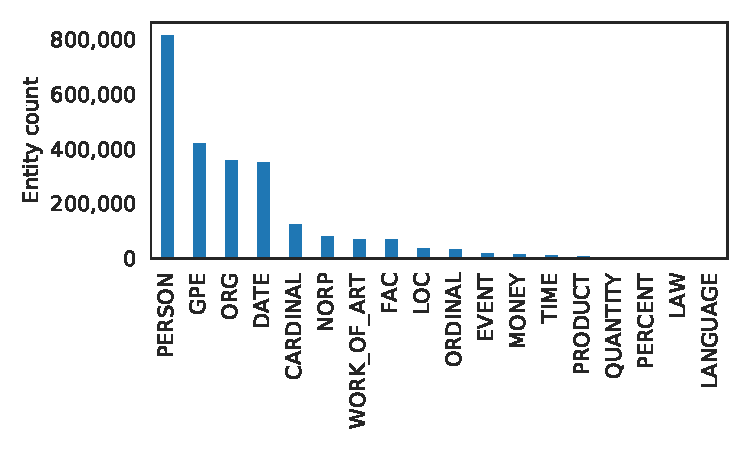
\includegraphics[width=0.99\linewidth]{figures/figure_2_entities.pdf}
   \end{center}
   \caption{Entity distribution in NYTimes800k training captions. The four
      most common entity types are people's names, geopolitical
      entities, organizations, and dates.}
   \label{fig:entities}
\end{figure}



\section{Further Experimental Results}

Table \ref{tab:results} reports BLEU-1, BLEU-2, BLEU-3,
BLEU-4~\cite{Papineni2002Bleu} ROUGE~\cite{Lin2004ROUGE},
METEOR~\cite{Denkowski2014Meteor}, and CIDEr~\cite{Vedantam2015CIDEr}. Our
results display a strong correlation between of all these metrics---a method
that performs well on one metric tends to perform well on them all. Of
particular interest is the CIDEr score since it uses Term Frequency Inverse
Document Frequency (TF-IDF) to put more importance on less common words such as
entity names. This makes CIDEr particularly well suited for evaluating news
captions where uncommon words tend to by vitally important, e.g. people's
names.

Table \ref{tab:results-names} further reports metrics on the entities. In
particular, we show the precision and recall of all proper nouns and new proper
nouns. We define a proper noun to be new if it has never appeared in any
training caption or article text. This is in contrast to the rare proper noun
metrics reported in the main paper, which are proper nouns that are not present
in any training caption but might have appeared inside a training article
context.

The three rightmost columns of Table \ref{tab:results-names} show the
linguistic quality metrics, including caption length (CL), type-token ratio
(TTR)~\cite{Templin1957CertainLS}, and Flesch readability ease
(FRE)~\cite{Flesch1948,Kincaid1975DerivationON}. The TTR is measured as
\begin{IEEEeqnarray}{lCl}
   \text{TTR} &=& \dfrac{U}{W}
\end{IEEEeqnarray}
where $U$ is the number of unique words and $W$ is the total number of words
in the caption. FRE is measured as
\begin{IEEEeqnarray}{lCl}
   \text{FRE} &=& 206.835-1.015\left({\frac {W}{S}}\right)-84.6\left({\frac {B}{W}}\right)
\end{IEEEeqnarray}
where $W$ is the number of words, $S$ is the number of sentences, and $B$ is
the number of syllables in the caption.

The higher TTR corresponds to a higher vocabulary variation in the text, while
a higher FRE indicates that the text uses simpler words and thus is easier to
read. Overall our models produce captions that are closer in length to the
ground truths than the previous state of the art \textit{Biten}
\cite{Biten2019GoodNews}. Moreover, our captions exhibit a level of language
complexity (as measured by Flesch score) that is closer to the ground truths.
However, there is still a gap in TTR, Flesch, and length, between captions
generated by our model and the human-written ground-truth captions.

Finally Figure~\ref{fig:chromati} and Figure~\ref{fig:sanders} show two
further set of generated captions.




\begin{table}[t] \caption {Model complexity. See Table 3 caption in the main
   paper for more explanation of each model variant.}
   \label{tab:models}
   \centering
   \begin{tabularx}{\linewidth}{Xc}
      \toprule
                                                   & No. of Parameters \\
      \midrule
      LSTM + GloVe + IA             & 157M              \\
      Transformer + GloVe + IA        & 148M              \\
      LSTM + RoBERTa + IA     & 159M              \\
      \midrule
      Transformer + RoBERTa                       & 125M              \\
      \quad + image attention (IA)          & 154M              \\
      \quad\quad + weighted RoBERTa                & 154M              \\
      \quad\quad\quad + location-aware             & 154M              \\
      \quad\quad\quad\quad + face attention        & 171M              \\
      \quad\quad\quad\quad\quad + object attention & 200M              \\
      \bottomrule
   \end{tabularx}
\end{table}


{\small
\bibliographystyle{ieee_fullname}
\bibliography{main}
}



\begin{table*}[p]
   \caption {BLEU, ROUGE, METEOR, and CIDEr metrics on the GoodNews and
      NYTimes800k datasets.}

   \label{tab:results}
   \centering
   \begin{tabularx}{\textwidth}{llXXXXXXX}
      \toprule
       &                                               & BLEU-1 & BLEU-2 & BLEU-3 & BLEU-4 & ROUGE & METEOR & CIDEr \\
      \midrule
      \multirow{10}{*}{\rotatebox[origin=c]{90}{GoodNews}}
       & Biten (Avg + CtxIns)~\cite{Biten2019GoodNews} & 9.04   & 3.66   & 1.71   & 0.89   & 12.2  & 4.37   & 13.1  \\
       & Biten (TBB + AttIns)~\cite{Biten2019GoodNews} & 8.10   & 3.26   & 1.48   & 0.76   & 12.2  & 4.17   & 12.7  \\
       \cmidrule{2-9}

       & LSTM + GloVe + IA              & 14.1   & 6.50   & 3.36   & 1.97   & 13.6  & 5.54   & 13.9  \\
        & Transformer + GloVe + IA         & 18.8   & 9.72   & 5.55   & 3.48   & 17.0  & 7.63   & 25.2  \\
        & LSTM + RoBERTa + IA      & 18.0   & 9.54   & 5.51   & 3.45   & 17.0  & 7.68   & 28.6  \\
      \cmidrule{2-9}

       & Transformer + RoBERTa                        & 19.7   & 11.3   & 6.96   & 4.60   & 18.6  & 8.82   & 40.9  \\
       & \quad + image attention           & 21.6   & 12.7   & 8.09   & 5.45   & 20.7  & 9.74   & 48.5  \\
       & \quad\quad + weighted RoBERTa                 & 22.3   & 13.4   & 8.72   & 6.0    & 21.2  & 10.1   & 53.1  \\
       & \quad\quad\quad + face attention              & \textbf{22.4}   & \textbf{13.5}   & 8.77   & \textbf{6.05}   & \textbf{21.4}  & 10.2   & \textbf{54.3}  \\
       & \quad\quad\quad\quad + object attention       & \textbf{22.4}   & \textbf{13.5}   & \textbf{8.80}   & \textbf{6.05}   & \textbf{21.4}  & \textbf{10.3}   & 53.8  \\
      \midrule
      \midrule \multirow{9}{*}{\rotatebox[origin=c]{90}{NYTimes800k}}

      & LSTM + GloVe + IA              & 13.4   & 6.0    & 3.06   & 1.77   & 13.1  & 5.34   & 12.1  \\
      & Transformer + GloVe + IA         & 16.8   & 8.28   & 4.56   & 2.75   & 15.9  & 6.94   & 20.3  \\
      & LSTM + RoBERTa + IA      & 17.0   & 8.92   & 5.19   & 3.29   & 16.1  & 7.31   & 24.9  \\
      \cmidrule{2-9}

       & Transformer + RoBERTa                        & 18.2   & 10.2   & 6.37   & 4.26   & 17.3  & 8.14   & 33.9  \\
       & \quad + image attention           & 20.0   & 11.6   & 7.38   & 5.01   & 19.4  & 9.05   & 40.3  \\
       & \quad\quad + weighted RoBERTa                 & 20.9   & 12.5   & 8.18   & 5.75   & 19.9  & 9.56   & 45.1  \\
       & \quad\quad\quad + location-aware              & 21.8   & 13.5   & 8.96   & 6.36   & 21.4  & 10.3   & 52.8  \\
       & \quad\quad\quad\quad + face attention         & \textbf{21.6}   & 13.3   & 8.85   & 6.26   & 21.5  & \textbf{10.3}   & 53.9  \\
       & \quad\quad\quad\quad\quad + object attention  & \textbf{21.6}   & \textbf{13.4}   & \textbf{8.90}   & \textbf{6.30}   & \textbf{21.7}  & \textbf{10.3}   & \textbf{54.4}  \\
      \bottomrule
   \end{tabularx}
\end{table*}

\begin{table*}[t]

   \caption {All proper noun and new proper noun precision (P) \& recall (R) on
      the GoodNews and NYTimes800k datasets. Linguistic measures on the
      generated captions: caption length (CL), type-token ratio (TTR), and
      Flesch readability ease (FRE).}

   \label{tab:results-names}
   \centering
   \begin{tabularx}{\textwidth}{llXXXXXX XXX}
      \toprule
       &                                               & \multicolumn{2}{c}{All proper nouns}
       & \multicolumn{2}{c}{New proper nouns}
       & \multirow{2}{*}{CL}                           & \multirow{2}{*}{TTR}                 & \multirow{2}{*}{FRE}                                    \\
       &                                               & P                                    & R                    & P    & R                         \\
      \midrule
      \multirow{8}{*}{\rotatebox[origin=c]{90}{GoodNews}}
       & Ground truths                                 & --                                   & --                   & --   & --   & 18.1 & 94.9 & 65.4 \\
      \cmidrule{2-9}
       & Biten (Avg + CtxIns)~\cite{Biten2019GoodNews} & 16.5                                 & 12.2                 & 2.70 & 12.0 & 9.89 & 92.2 & 78.3 \\
       & Biten (TBB + AttIns)~\cite{Biten2019GoodNews} & 19.2                                 & 11.0                 & 4.21 & 12.3 & 9.14 & 90.7 & 77.6 \\
       \cmidrule{2-9}

       & LSTM + GloVe + IA              & 16.1                                 & 11.3                 & 0    & 0    & 14.0 & 89.5 & 77.2 \\
        & Transformer + GloVe + IA         & 22.7                                 & 18.4                 & 0    & 0    & 16.0 & 88.4 & 73.9 \\
        & LSTM + RoBERTa + IA      & 25.1                                 & 20.8                 & 1.68 & 7.86 & 15.0 & 89.0 & 75.7 \\
      \cmidrule{2-9}

       & Transformer + RoBERTa                        & 30.7                                 & 26.0                 & 7.69 & 16.4 & 15.1 & 90.0 & 73.0 \\
       & \quad + image attention           & 33.4                                 & 28.0                 & 8.53 & 19.3 & 15.2 & 90.0 & 72.5 \\
       & \quad\quad + weighted RoBERTa                 & 33.9                                 & 29.6                 & \textbf{15.2} & \textbf{24.4} & 15.5 & 90.8 & 71.8 \\
       & \quad\quad\quad + face attention              & 34.3                                 & 29.8                 & 13.6 & 22.2 & 15.4 & 90.8 & 71.8 \\
       & \quad\quad\quad\quad + object attention       & \textbf{34.7}                                 & \textbf{29.9}                 & 13.3 & 23.6 & 15.3 & 90.9 & 72.0 \\
      \midrule
      \midrule
      \multirow{7}{*}{\rotatebox[origin=c]{90}{NYTimes800k}}
       & Ground truths                                 & --                                   & --                   & --   & --   & 18.4 & 94.6 & 63.9 \\
      \cmidrule{2-9}

      & LSTM + GloVe + IA              & 15.8                                 & 12.4                 & 0    & 0    & 13.9 & 88.7 & 76.1 \\
      & Transformer + GloVe + IA         & 21.5                                 & 18.2                 & 0    & 0    & 14.8 & 88.8 & 71.9 \\
      & LSTM + RoBERTa + IA      & 24.1                                 & 21.8                 & 3.28 & 7.18 & 14.8 & 89.3 & 73.3 \\
      \cmidrule{2-9}
       & Transformer + RoBERTa                        & 28.0                                 & 26.0                 & 13.4 & 14.5 & 15.2 & 90.4 & 71.4 \\
       & \quad + image attention           & 31.1                                 & 28.7                 & 15.6 & 17.2 & 15.1 & 90.1 & 71.5 \\
       & \quad\quad + weighted RoBERTa                 & 31.8                                 & 30.5                 & 21.7 & 20.2 & 15.5 & 91.6 & 70.1 \\
       & \quad\quad\quad + location-aware              & 36.4                                 & 34.1                 & 26.3 & \textbf{25.3} & 15.1 & 91.7 & 70.8 \\
       & \quad\quad\quad\quad + face attention         & 36.8                                 & 34.2                 & 26.2 & 24.2 & 14.9 & 91.8 & 70.9 \\
       & \quad\quad\quad\quad\quad + object attention  & \textbf{37.2}                                 & \textbf{34.5}                 & \textbf{26.7} & 25.1 & 14.8 & 91.9 & 71.2 \\
      \bottomrule
   \end{tabularx}
\end{table*}

\begin{table*}[t]

   \caption {Geopolitical entity (GPE), organization (ORG), and date (DATE)
      precision (P) \& recall (R) on the GoodNews and NYTimes800k datasets.}

   \label{tab:gpe-org-date}
   \centering
   \begin{tabularx}{\textwidth}{llXXXXXX}
      \toprule
       &                                               & \multicolumn{2}{c}{GPE} & \multicolumn{2}{c}{ORG} & \multicolumn{2}{c}{DATE}                      \\
       &                                               & P                       & R                       & P                        & R    & P    & R    \\
      \midrule
      \multirow{8}{*}{\rotatebox[origin=c]{90}{GoodNews}}
       & Biten (Avg + CtxIns)~\cite{Biten2019GoodNews} & 12.0                    & 11.5                    & 5.67                     & 7.45 & 6.12 & 4.03 \\
       & Biten (TBB + AttIns)~\cite{Biten2019GoodNews} & 12.8                    & 8.41                    & 5.81                     & 7.36 & 5.86 & 4.06 \\
       \cmidrule{2-8}

       & LSTM + GloVe + IA              & 15.6                    & 12.8                    & 14.0                     & 8.58 & 11.0 & 8.20 \\
        & Transformer + GloVe + IA         & 20.8                    & 18.8                    & 16.6                     & 11.8 & 12.0 & 10.1 \\
        & LSTM + RoBERTa + IA      & 20.8                    & 19.2                    & 16.9                     & 12.3 & 13.4 & 10.9 \\
      \cmidrule{2-8}

       & Transformer + RoBERTa                        & 22.6                    & 22.5                    & 20.4                     & 16.3 & 13.8 & 12.6 \\
       & \quad + image attention           & \textbf{25.8}                    & 24.5                    & 21.0                     & 17.3 & 14.4 & 13.0 \\
       & \quad\quad + weighted RoBERTa                 & 25.0                    & 24.2                    & 22.0                     & \textbf{18.7} & 14.3 & 13.1 \\
       & \quad\quad\quad + face attention              & 24.9                    & 24.4                    & 21.6                     & 18.5 & 14.7 & \textbf{13.3} \\
       & \quad\quad\quad\quad + object attention       & 25.6                    & \textbf{24.7}                    & \textbf{22.4}                     & \textbf{18.7} & \textbf{15.1} & \textbf{13.3} \\
      \midrule
      \midrule
      \multirow{7}{*}{\rotatebox[origin=c]{90}{NYTimes800k}}
      & LSTM + GloVe + IA              & 16.0                    & 14.7                    & 8.60                     & 4.89 & 11.3 & 8.31 \\
      & Transformer + GloVe + IA         & 19.1                    & 21.8                    & 12.1                     & 7.95 & 11.3 & 10.1 \\
      & LSTM + RoBERTa + IA      & 20.2                    & 22.2                    & 13.1                     & 8.95 & 11.8 & 11.1 \\
      \cmidrule{2-8}
       & Transformer + RoBERTa                        & 21.4                    & 25.4                    & 15.8                     & 12.2 & 12.0 & 12.5 \\
       & \quad + image attention           & 23.9                    & 27.3                    & 17.6                     & 13.6 & 12.8 & 13.2 \\
       & \quad\quad + weighted RoBERTa                 & 24.2                    & 28.2                    & 19.2                     & 15.6 & 13.9 & 14.3 \\
       & \quad\quad\quad + location-aware              & 26.8                    & 30.1                    & 20.9                     & \textbf{17.3} & \textbf{14.1} & \textbf{14.1} \\
       & \quad\quad\quad\quad + face attention         & \textbf{26.9}                    & \textbf{30.6}                    & 20.7                     & 16.5 & 13.9 & \textbf{14.1} \\
       & \quad\quad\quad\quad\quad + object attention  & 26.8                    & \textbf{30.6}                    & \textbf{21.9}                     & 17.2 & 13.7 & 13.8 \\

      \bottomrule
   \end{tabularx}
\end{table*}

\clearpage


\begin{figure*}[p]
   \begin{center}
      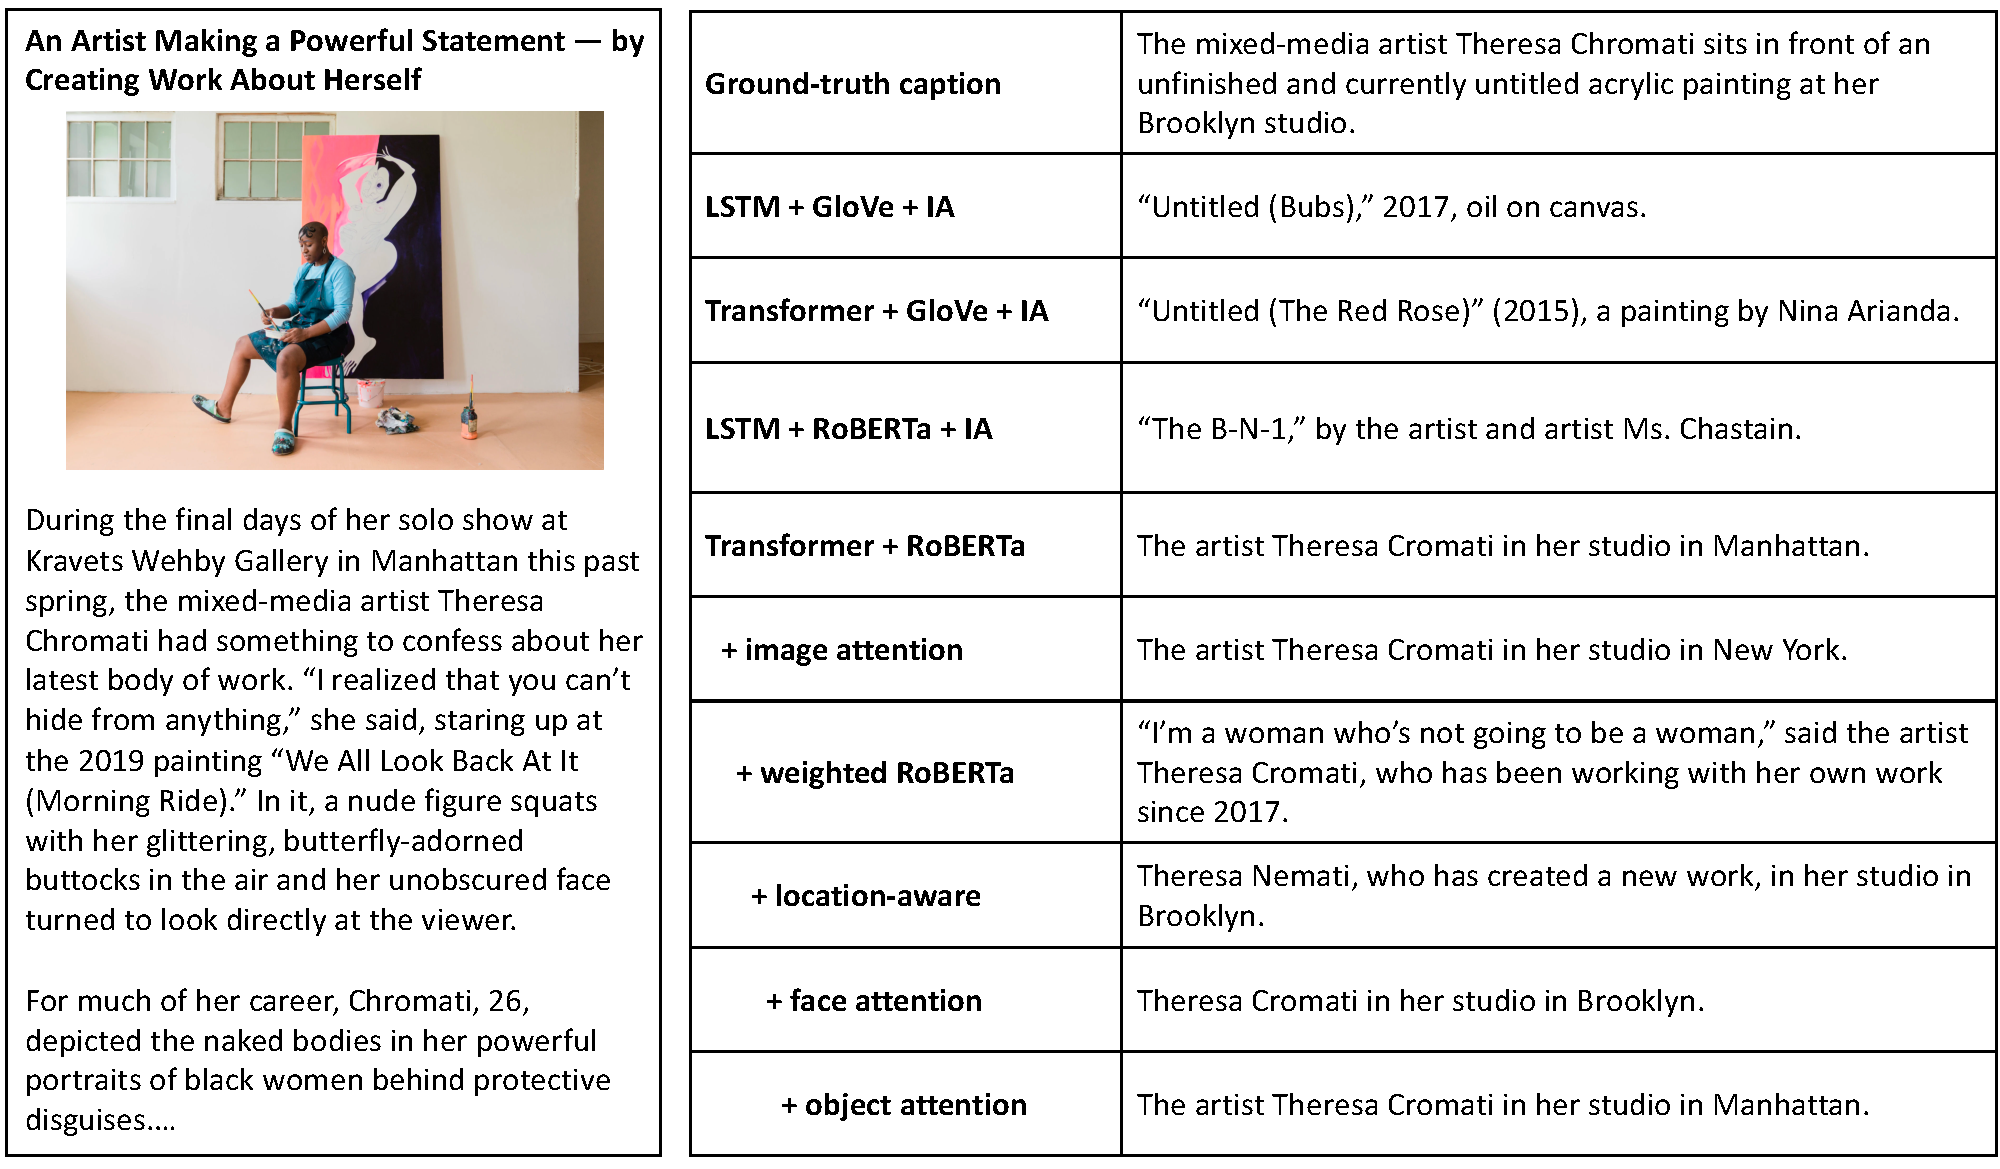
\includegraphics[width=\linewidth]{figures/chromati.pdf}
   \end{center}
   \caption{An example article (left) and the corresponding news captions
      (right) from the NYTimes800k test set. The name ``Chromati" has never
      appeared in the training data, and none of the models can spell the
      artist's name correctly. They all miss the letter ``h'' in her name.
      Captions from models that use an LSTM or GloVe contain made-up names for
      both the painting and the artist. Finally the model that has no access to
      the image, \textit{Transformer + RoBERTa}, still guesses correctly that
      the image is about the artist being in her studio. This shows that
      NYTimes article images can have a predictable theme.}
   \label{fig:chromati}
\end{figure*}

\begin{figure*}[p]
   \begin{center}
      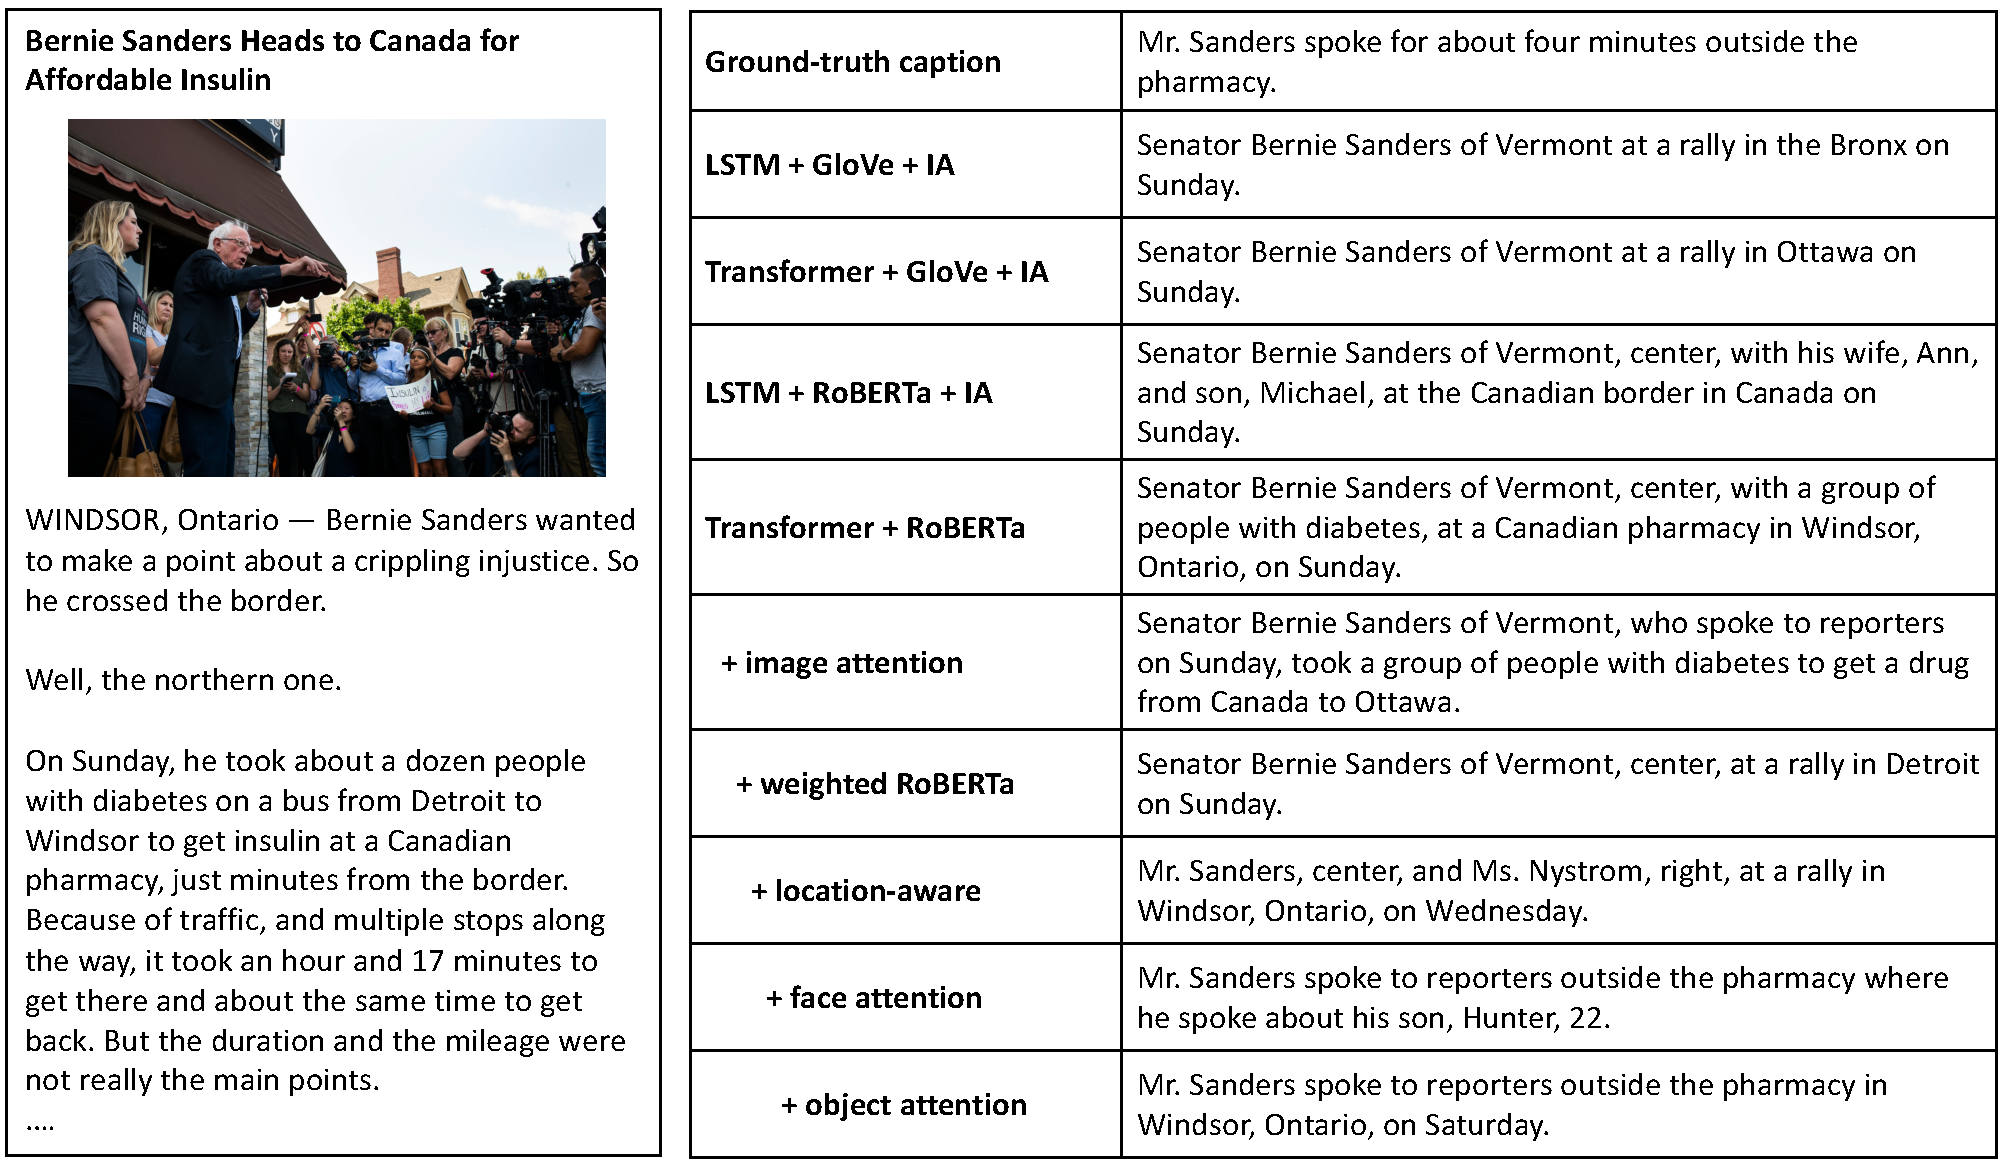
\includegraphics[width=\linewidth]{figures/sanders.pdf}
   \end{center}
   \caption{An example article (left) and the corresponding news captions
      (right) from the NYTimes800k test set. The model that has no access to
      the image, \textit{Transformer + RoBERTa}, is correct in predicting that
      the image is about Bernie Sanders. However it guesses that he is with a
      group of people with diabetes, which is not correct but is sensible given
      the article content. Some of the models manage to override the strong
      prior that he is at a rally (which is what many of Bernie Sanders images
      in the training set are about) and correctly say that he is outside a
      pharmacy. The caption from the model with object attention is the most
      accurate because it generates all three entities correctly: Windsor in
      Ontario, the reporters, and the pharmacy. }
   \label{fig:sanders}
\end{figure*}


\end{document}
